\section{Front-end}

En esta sección se detallan cada uno de los escenarios con los que cuenta 
la solución, incluyendo la retroalimentación y el registro de las actividades del 
usuario.

Las descripciones a continuación están agrupadas por los escenarios principales.

\subsection{Pantalla de inicio}

La solución se inicia con un escenario que está inspirado en el laboratorio de
enfermería del \Gls{iab}, es la primera experiencia que tiene el usuario al
utilizar la misma, sirve como un menú principal, desde este punto todas las
opciones son accesibles para el usuario como se puede observar en la
figura~\ref{fig:pantalla_inicio}, este escenario es denominado~\emph{Inicio}.

Al instalar la solución se muestra una pequeña ventana solicitando el número de
teléfono del usuario, se utiliza esta información como un identificador del
usuario para asociar la información del mismo con un alumno en
particular.

\begin{figure}[H] 
\centering 
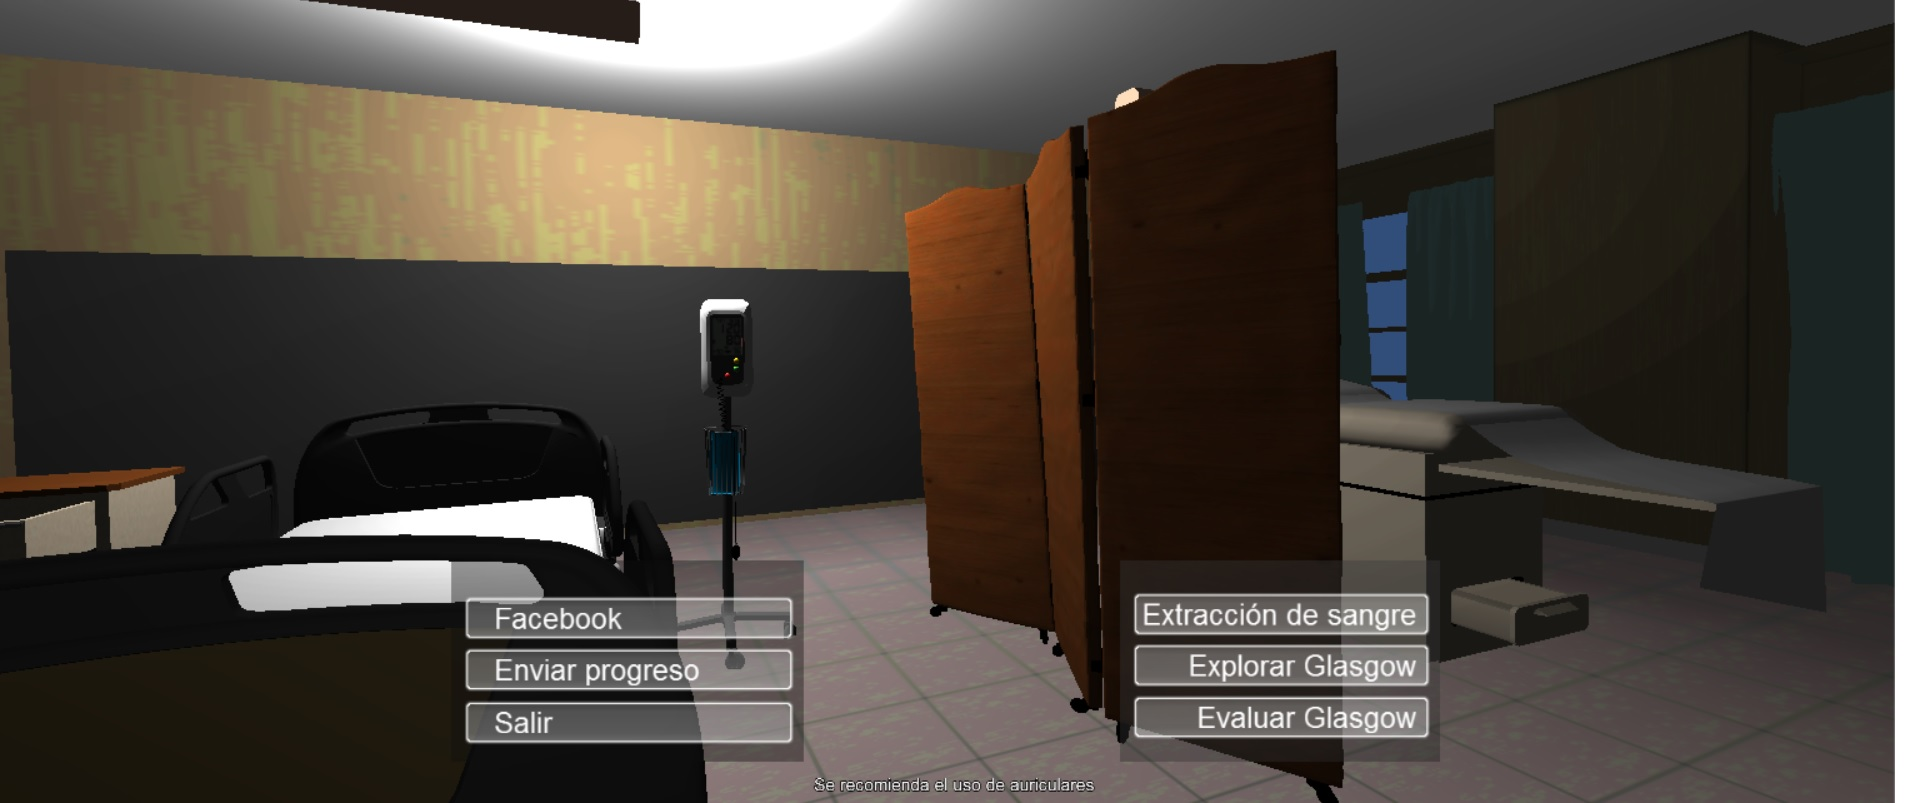
\includegraphics[width=10cm]{solucion/images/pantalla_inicio.jpg}
\caption{Pantalla de inicio de la solución con todas las opciones disponibles.}
\label{fig:pantalla_inicio}
\end{figure}

La sala de hospital mostrada como fondo en la figura~\ref{fig:pantalla_inicio}
es la que se utiliza como escenografía principal en las escenas de los
procedimientos. Mientras se muestran las opciones, se ejecuta una animación que
recorre el escenario mostrando los detalles importantes, como la camilla, el
lector de estadísticas vitales, y demás elementos del escenario.

Las opciones disponibles en la pantalla de inicio son:

\begin{itemize}
\item \enquote{Enviar Progreso}: esta función envía toda la información
    acerca de la actividad que el usuario realizó en la aplicación a un servidor
    \emph{back-end} que se encarga de almacenar estos datos.
\item \enquote{Salir de la simulación}: esta función permite salir de la
    aplicación.
\item Botón \enquote{Facebook}: esta función permite al usuario ingresar a su
    cuenta de Facebook.
\item \enquote{Extracción de sangre}: esta función permite ingresar a la
    escena correspondiente al procedimiento de venopunción 
    permitiendo al usuario jugar una nueva partida.
\item \enquote{Explorar Glasgow}: esta función permite ingresar a la
    escena correspondiente al procedimiento para explorar las reacción de un
    paciente con un diagnóstico específico de la escala de Glasgow permitiendo
    al usuario jugar una nueva partida.
\item \enquote{Evaluar Glasgow}: esta función permite ingresar a la escena
    correspondiente al procedimiento de valoración de la
    escala de Glasgow para un paciente con estado aleatorio permitiendo al
    usuario jugar una nueva partida.
\end{itemize}


\subsection{Venopunción}

Al seleccionar el procedimiento de venopunción o extracción de sangre, en la pantalla de inicio,  
la aplicación inmediatamente muestra el escenario del procedimiento como se puede 
observar en la figura~\ref{fig:hemocultivo_principal}. 

\begin{figure}[H] 
\centering 
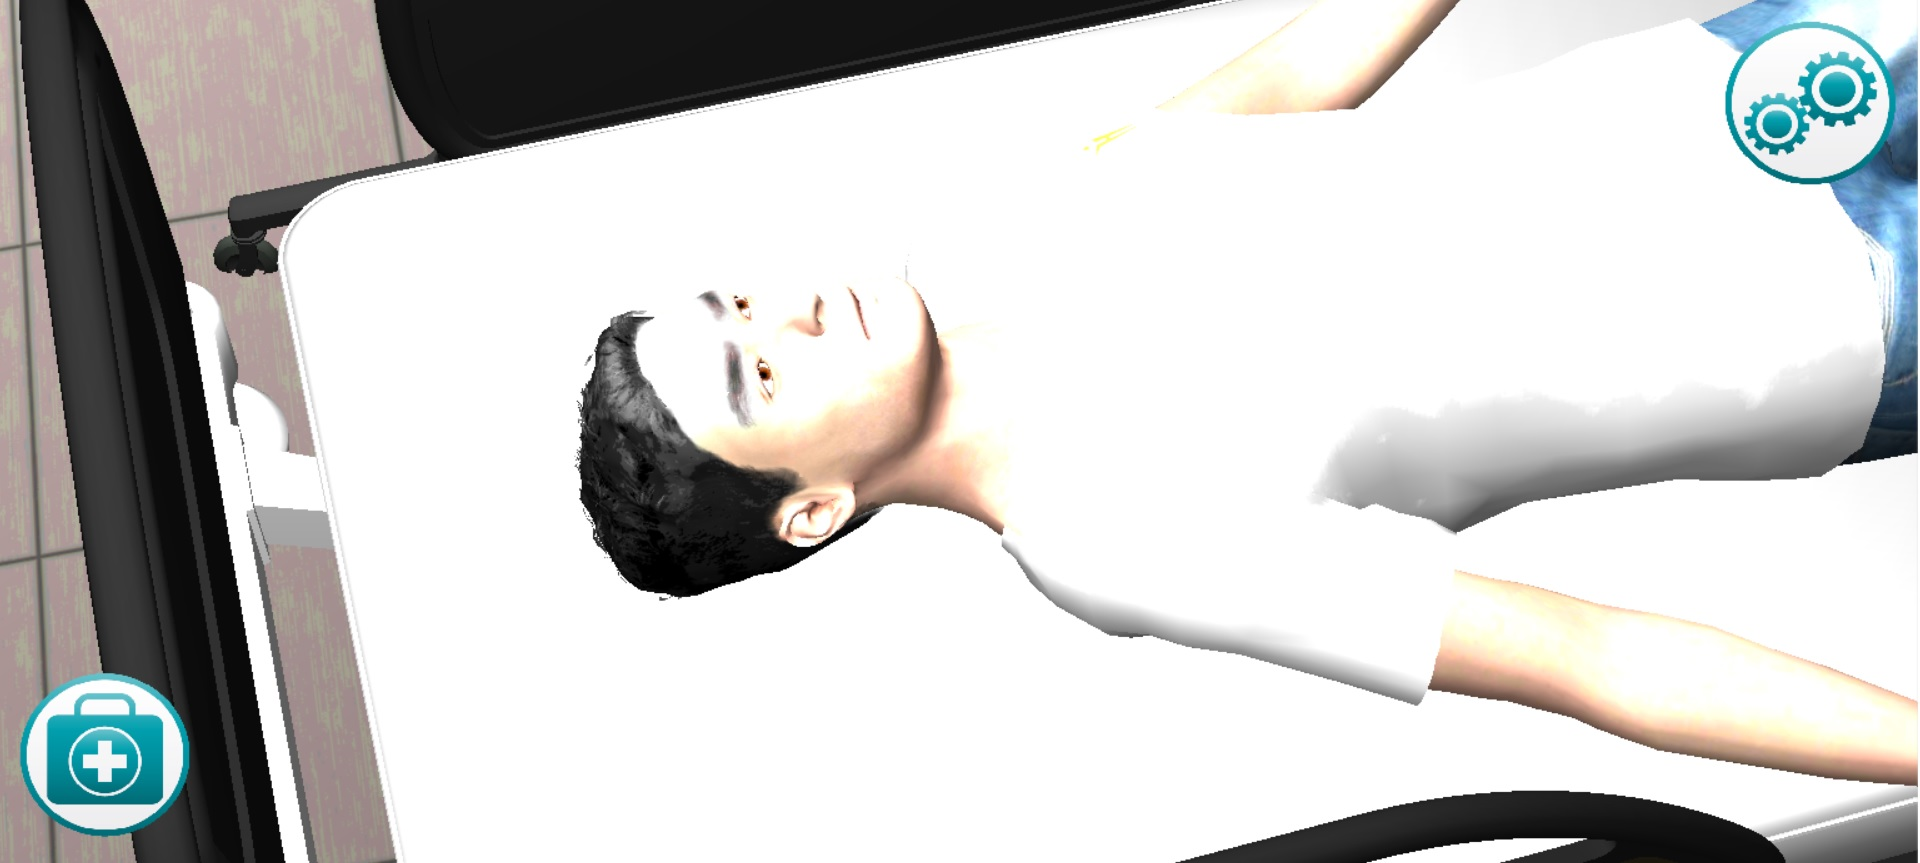
\includegraphics[width=10cm]{solucion/images/hemocultivo_principal.jpg}
\caption{Pantalla principal de la escena del procedimiento de extracción de sangre.}
\label{fig:hemocultivo_principal}
\end{figure}

La posición inicial de la cámara se ubica en un ángulo donde se puedan ver 
bien los brazos del paciente para facilitar al usuario la realización del 
procedimiento.

A continuación se detallan cada una de las opciones y formas disponibles de
interactuar con el escenario del procedimiento.


\subsubsection{Entidades}

Existen dos entidades principales, cada entidad mantiene un estado independiente 
de la otra. Estas entidades son:

\begin{itemize}

\item \textbf{Paciente:} es una entidad con estado complejo, el cual es
    constantemente modificado por las acciones del usuario, en resumen, la
    información que contiene el paciente es:
    \begin{itemize}
        \item Jeringas\footnote{No se limita la cantidad de jeringas que un
                paciente pueda tener insertadas en un momento dado.}.
        \item Estado de las manos (abiertas o cerradas).
        \item Torniquetes.
        \item Zonas esterilizadas.
        \item Zonas presionadas.
    \end{itemize}

\item \textbf{Usuario:} mantiene un estado en todo momento del cual dependen sus
    acciones. Por ejemplo, si la mano del enfermero no está esterilizada,
    cualquier interacción con el paciente provocará que el paciente se
    contamine. La información que contiene la entidad usuario es:

    \begin{itemize}
    \item Estado de las manos.
    \item Estado de la vestimenta (guantes, bata, tapaboca y gorro).
    \item Elemento en uso.
    \end{itemize}
\end{itemize}

\subsubsection{Interacción con la interfaz de usuario}

La interfaz principal de este escenario posee dos menús como se indica en la
figura~\ref{fig:hemocultivo_gui} con los números $1$ y $2$, las opciones dentro
cada menú poseen una imagen intuitiva que representa la función que realizan. Al
menú número 1 lo llamaremos \emph{Elementos} y al número 2 \emph{Opciones}.

\begin{figure}[H]
\centering
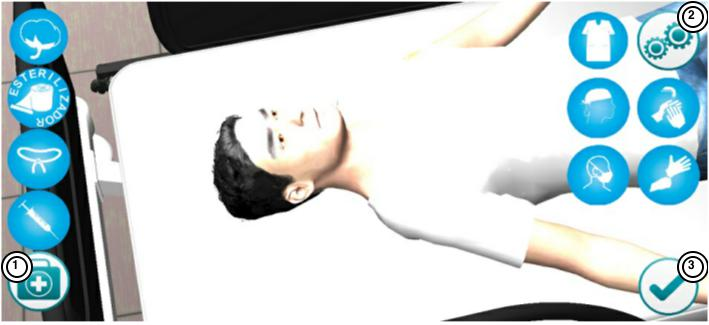
\includegraphics[width=10cm]{solucion/images/hemocultivo_menus.jpg}
\caption{Vista de la interfaz principal del escenario \emph{Extracción de
        sangre}, con todas las opciones desplegadas.}
\label{fig:hemocultivo_gui}
\end{figure}

Adicionalmente, existen dos tipos de indicadores mostrados en la
figura~\ref{fig:hemocultivo_seleccion}. El tipo de indicador marcado con el número $1$
representa el elemento actualmente seleccionado y el tipo de indicador marcado
con el número $2$ representa al estado actual del usuario o enfermero en cuanto a
aspectos de bioseguridad referentes a vestimentas de protección personal.

\begin{figure}[H]
\centering
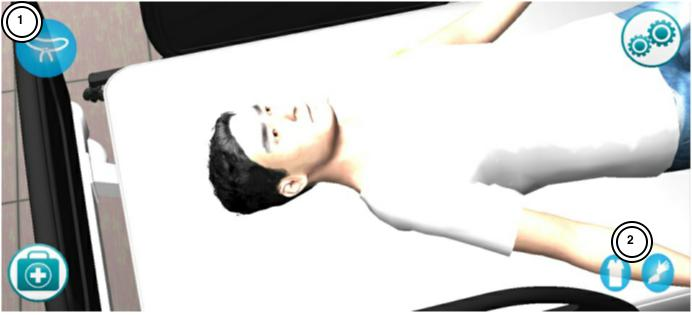
\includegraphics[width=10cm]{solucion/images/hemocultivo_seleccion.jpg}
\caption{Indicadores de selección de elementos y de estado de usuario o enfermero.}
\label{fig:hemocultivo_seleccion}
\end{figure}

\begin{itemize}
\item \textbf{Menú de opciones}

Cuando el usuario presiona el menú \emph{Opciones} se le muestra las distintas acciones que puede
realizar en cuanto a aspectos de bioseguridad, todos los botones
afectan al estado del usuario o enfermero. %Con excepción del lavado de manos,
%las opciones disponibles representan el hecho de ponerse/sacarse los guantes, el
%tapaboca, el gorro y la bata, esto se da seleccionando/deseleccionando estas
%opciones. 
Además se brinda la opción de finalizar la partida con el botón
indicado en la figura~\ref{fig:hemocultivo_gui} con el número $3$.

\item \textbf{Menú de elementos}

En el menú \emph{Elementos} se despliegan opciones que representan a los
elementos que se utilizan para realizar el procedimiento, una vez presionado un
elemento queda seleccionado (simulando que es la herramienta que el enfermero
tiene en la mano en ese momento), sólo un elemento puede ser seleccionado a la
vez. Si el mismo botón se vuelve a presionar inmediatamente después de haber
sido presionado, el elemento se des-selecciona (simulando que el enfermero dejó
la herramienta). Los elementos disponibles están enumerados en la
figura~\ref{fig:hemocultivo_elementos} y son los siguientes:


\begin{figure}[H]
\centering
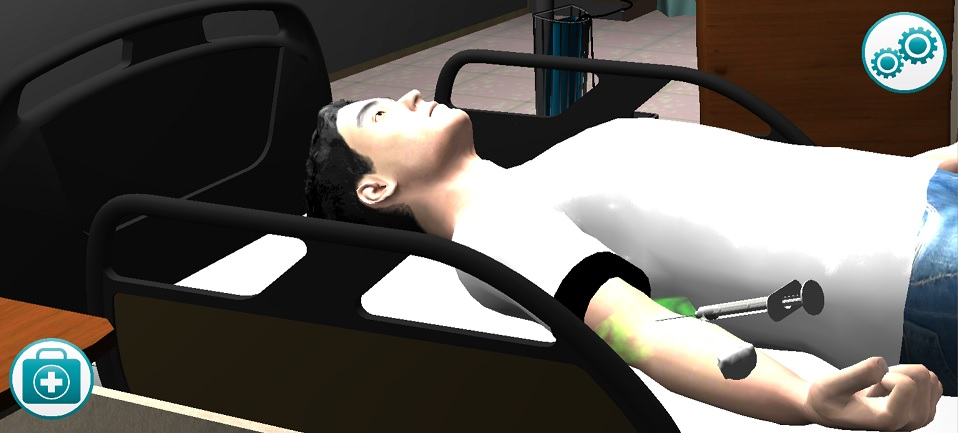
\includegraphics[width=10cm]{solucion/images/hemocultivo_elementos.jpg}
\caption{Interfaz con los elementos en el paciente.}
\label{fig:hemocultivo_elementos}
\end{figure}


\begin{enumerate} 
    
\item \textbf{Torniquete}: es el primer elemento que se debe usar, para
    utilizarlo, se debe presionar una zona del brazo del paciente, en ese
    momento, el torniquete aparece en ese lugar, para extraerlo, se debe
    presionar el torniquete y elegir la opción extraer en un menú que aparecerá
    inmediatamente.

\item \textbf{Esterilizador}: es un elemento que se utiliza para realizar la
    higienización del punto de punción, para utilizarlo se debe presionar
    cualquier zona del brazo del paciente, a continuación aparece una gaza, la
    cual debe ser agitada con un dedo durante un segundo para que se cree una
    zona estéril, la zona estéril creada, es visible a través de una cápsula.

\item \textbf{Jeringa}: es el elemento utilizado para realizar la extracción, su
    utilización es similar a la del \emph{Torniquete}.

    A través de un menú contextual, se ofrece la posibilidad de realizar un
    acercamiento, como se observa en la
    figura~\ref{fig:hemocultivo_jeringa_zoom}, en la vista ampliada. Se puede
    realizar la extracción de sangre utilizando dos dedos, con el primero se
    presiona el tambor y con el segundo dedo se extrae el émbolo\footnote{El
        tambor es la parte de la jeringa que almacena el fluido, mientras que el
        émbolo es la parte que se utiliza para presionar o succionar el fluido}.
    
\item \textbf{Algodón}: el algodón se utiliza para presionar una zona que
    recientemente fue punzada, para utilizar este elemento, basta con presionar
    el brazo del paciente durante un segundo.

\end{enumerate}

\begin{figure}[H]
\centering 
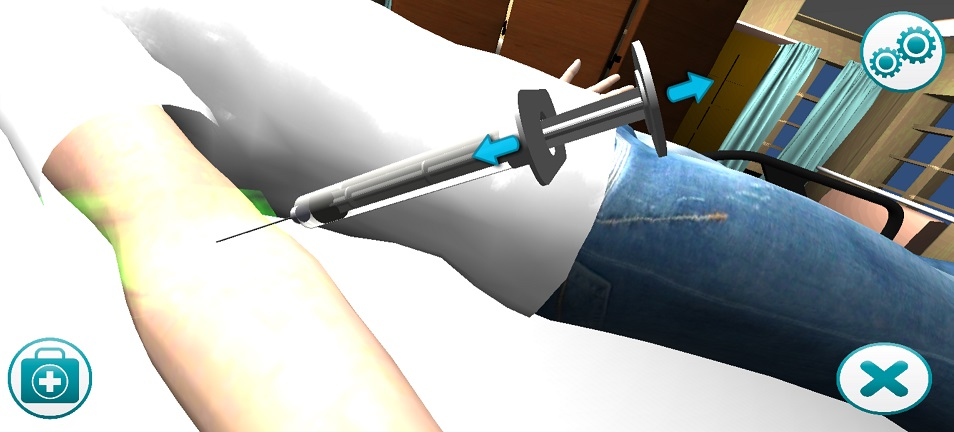
\includegraphics[width=10cm]{solucion/images/hemocultivo_jeringa_ampliada.jpg}
\caption{Vista de la jeringa ampliada, facilitando la extracción de sangre. Se
    agregan flechas azules para facilitar la comprensión de cómo se extrae
    sangre.}
\label{fig:hemocultivo_jeringa_zoom}
\end{figure}


Para la utilización de los elementos, existe un menú contextual\footnote{Un menú
    que se despliega al presionar un elemento, es contextual pues varía de
    acuerdo al elemento seleccionado.}, que lista las opciones disponibles por
elemento, como se observa en la figura~\ref{fig:hemocultivo_torniquete_cm}.

\begin{figure}[H]
\centering
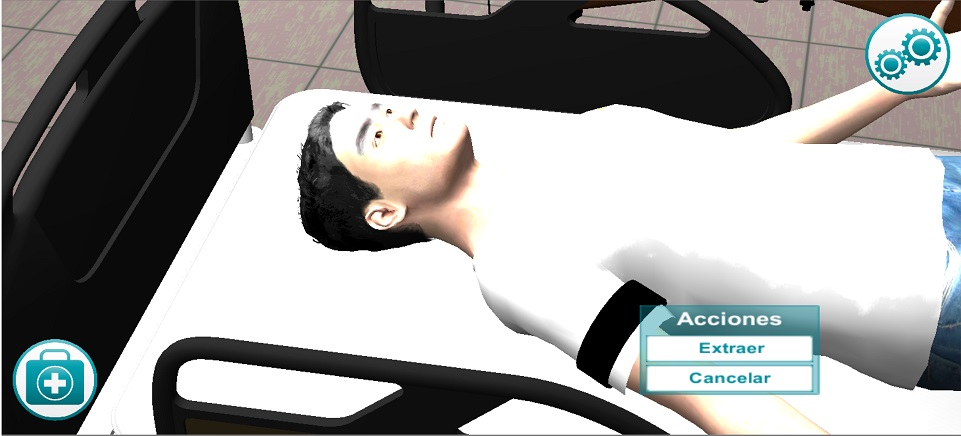
\includegraphics[width=10cm]{solucion/images/hemocultivo_contextual.jpg}
\caption{Menú contextual del elemento torniquete.}
\label{fig:hemocultivo_torniquete_cm}
\end{figure}


\item \textbf{Menú de comandos de voz}

Por último, la solución también cuenta con un menú que presenta una serie de órdenes 
de voz como se observa en la figura~\ref{fig:hemocultivo_voz_gui}. Este menú se 
	activa y se muestra en pantalla cuando la solución detecta que el usuario ha 
	hablado. Las opciones disponibles son las siguientes:
	
	\begin{itemize}
	\item Explicar procedimiento.
	\item Abrir la mano izquierda.
	\item Abrir la mano derecha.
	\item Cerrar la mano izquierda.
	\item Cerrar la mano derecha.
	\end{itemize}
	
	Estas opciones, a excepción de \emph{Explicar procedimiento}, provocan que el 
	paciente realice la petición realizada. De esta manera se simula una conversación 
	entre el usuario y el paciente.
	
	\begin{figure}[H]
	\centering
	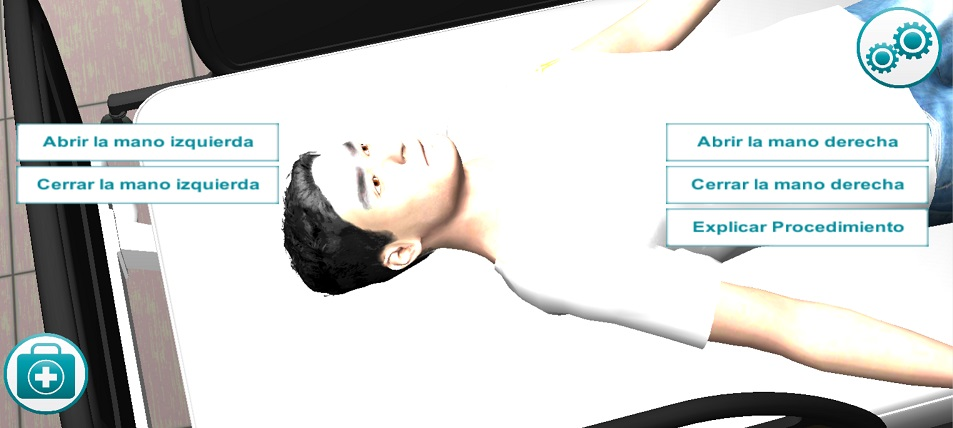
\includegraphics[width=10cm]{solucion/images/hemocultivo_comando_voz.jpg}
	\caption{Opciones mostradas al detectar sonido en la escena de extracción
    de sangre.}
	\label{fig:hemocultivo_voz_gui}
	\end{figure}

\end{itemize}

%\observacion{Pulir el párrafo siguiente}








%\subsubsection{Acciones}
%\observacion{Sean consistentes con las terminologías}
%
%Los usuarios pueden interactuar con el paciente virtual de tres formas, por
%\emph{comandos de voz} que simulan una conversación entre el paciente y
%enfermero, por \emph{las opciones}, que engloban las acciones que puede realizar un
%enfermero en cuanto a bioseguridad, y por \emph{los elementos} que son las
%herramientas que puede utilizar el enfermero durante un procedimiento.
%
%\begin{itemize}
%\item{\textbf{Comando de voz}}
%
%	Se implementa un menú que presenta una serie de órdenes de voz como se observa en la figura~\ref{fig:hemocultivo_voz_gui}. Este menú se 
%	activa y se muestra en pantalla cuando la solución detecta que el usuario ha 
%	hablado. Las opciones disponibles son las siguientes:
%	
%	\begin{itemize}
%	\item Explicar procedimiento.
%	\item Abrir la mano izquierda.
%	\item Abrir la mano derecha.
%	\item Cerrar la mano izquierda.
%	\item Cerrar la mano derecha.
%	\end{itemize}
%	
%	Estas opciones, a excepción de \emph{Explicar procedimiento}, provocan que el 
%	paciente realice la petición realizada. De esta manera se simula una conversación 
%	entre el usuario y el paciente.
%
%\begin{figure}[H]
%\centering
%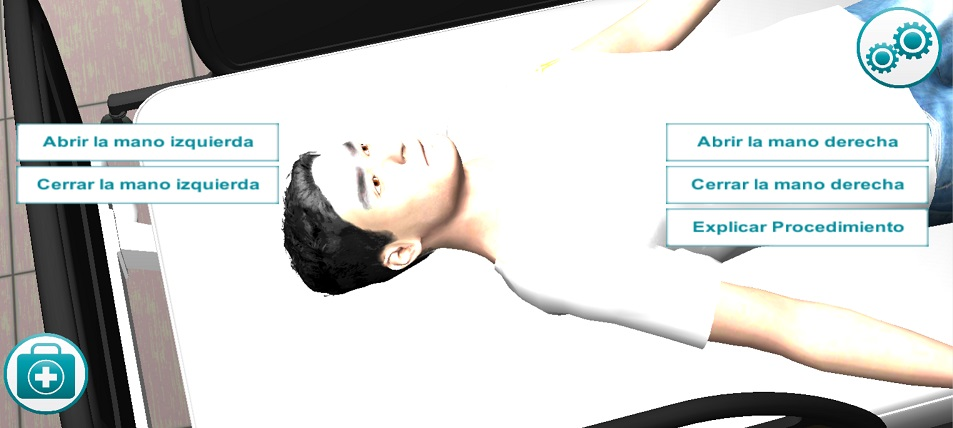
\includegraphics[width=10cm]{solucion/images/hemocultivo_comando_voz.jpg}
%\caption{Opciones mostradas al detectar sonido en la escena de extracción
%    de sangre.}
%\label{fig:hemocultivo_voz_gui}
%\end{figure}
%
%
%
%\item{\textbf{Opciones}}
%
%Las \emph{Opciones} representan las acciones que puede realizar el usuario haciendo uso de las opciones  
%disponibles en el menú indicado por el número 2 en la figura~\ref{fig:hemocultivo_menus}. Estas 
%opciones afectan al estado de la entidad \emph{enfermero} y representan a los aspectos de 
%bioseguridad como el lavado de manos, en calzado de guantes, entre otros.
%
%\begin{figure}[H]
%\centering
%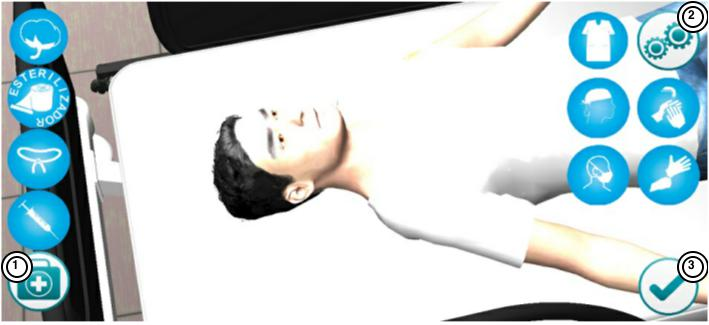
\includegraphics[width=10cm]{solucion/images/hemocultivo_menus.jpg}
%\caption{Menús de la escena principal del procedimiento de venopunción.}
%\label{fig:hemocultivo_menus}
%\end{figure}
%
%%Las \emph{Opciones} son aquellas acciones que puede realizar el usuario y afectan
%%únicamente al paciente. Representan a los aspectos de bioseguridad, es decir,
%%acciones como lavarse las manos, calzarse guantes, gorro, bata y tapaboca.
%%
%%Estas opciones afectan al estado de la entidad \emph{enfermero}.
%
%\item{\textbf{Elementos}}
%
%Los \emph{Elementos} representan las herramientas que utiliza un enfermero
%durante el procedimiento, un solo elemento puede ser utilizado en cualquier
%momento. Las opciones disponibles se pueden ver en el menú marcado por el número 1 
%en la figura~\ref{fig:hemocultivo_menus}. 
%
%
%%\observacion{Desconectado?}
%%\observacion{Falta una intro a todo esto (se refiere a los elementos, y a la
%%    descripción de la imagen~\ref{fig:hemocultivo_voz_gui})}
%\begin{figure}[H]
%\centering
%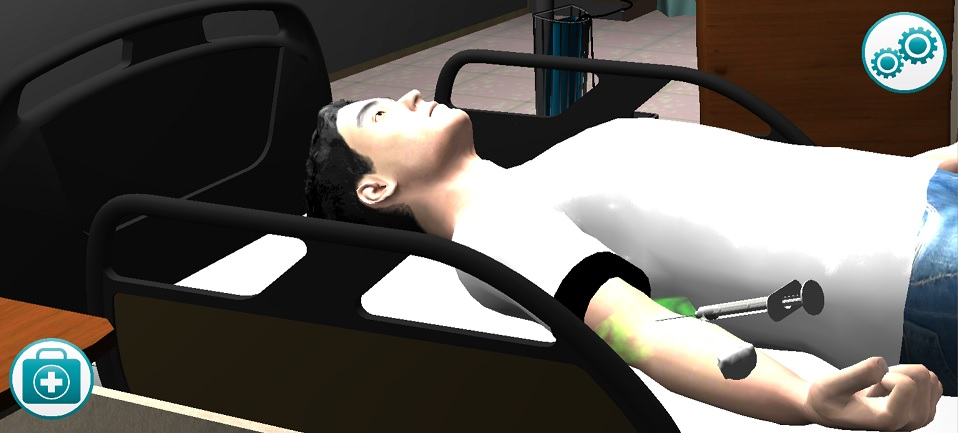
\includegraphics[width=10cm]{solucion/images/hemocultivo_elementos.jpg}
%\caption{Interfaz con los elementos en el paciente.}
%\label{fig:hemocultivo_elementos}
%\end{figure}
%
%Los elementos enumerados en la figura~\ref{fig:hemocultivo_elementos}, son:
%
%\begin{enumerate}
%\item \textbf{Torniquete}: es el primer elemento que se debe usar, para
%    utilizarlo, se debe presionar una zona del brazo del
%    paciente, en ese momento, el torniquete aparece en ese lugar, para
%    extraerlo, se debe presionar el torniquete y elegir la opción extraer en un menú 
%    que aparecerá inmediatamente.
%
%\item \textbf{Esterilizador}: es un elemento que se utiliza para realizar la
%    higienización del punto de punción, para utilizarlo se debe presionar
%    cualquier zona del brazo del paciente, a continuación aparece una gaza, la
%    cual debe ser agitada con un dedo durante un segundo para que se cree una
%    zona estéril, la zona estéril creada, es visible a través de una cápsula.
%
%\item \textbf{Jeringa}: es el elemento utilizado para realizar la extracción, su
%    utilización es similar a la del \emph{Torniquete}.
%
%    A través de un menú contextual, se ofrece la posibilidad de realizar un
%    acercamiento, como se observa en la figura~\ref{fig:hemocultivo_jeringa_zoom}, 
%    en la vista ampliada. Se puede realizar la extracción de sangre utilizando dos dedos, 
%    con el primero se presiona el tambor y con el segundo dedo se extrae el émbolo\footnote{El
%    tambor es la parte de la jeringa que almacena el fluido, mientras que el
%    émbolo es la parte que se utiliza para presionar o succionar el fluido}.
%    
%\item \textbf{Algodón}: el algodón se utiliza para presionar una zona que
%    recientemente fue punzada, para utilizar este elemento, basta con presionar
%    el brazo del paciente durante un segundo.
%
%\end{enumerate}
%
%
%\begin{figure}[H]
%\centering 
%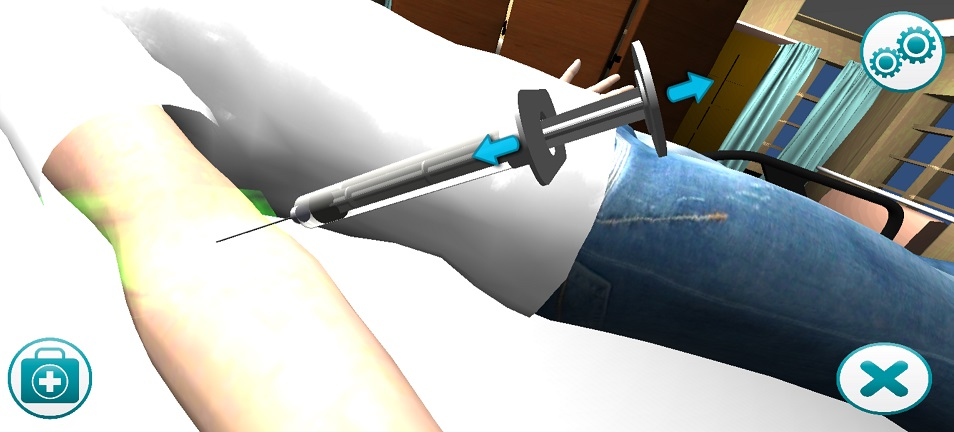
\includegraphics[width=10cm]{solucion/images/hemocultivo_jeringa_ampliada.jpg}
%\caption{Vista de la jeringa ampliada, facilitando la extracción de sangre. Se
%    agregan flechas azules para facilitar la comprensión de cómo se extrae
%    sangre.}
%\label{fig:hemocultivo_jeringa_zoom}
%\end{figure}
%
%\end{itemize}

\subsubsection{Evaluación al usuario}

Para realizar la evaluación del usuario en el procedimiento de \emph{Venopunción} 
se utiliza un motor de \Gls{eca}, las características de estos motores están descritas 
en la sección~\ref{sec:eca}.

Definir si las acciones de un usuario son correctas utilizando un motor 
\Gls{eca} es sencillo teniendo en cuenta que sólo se deben definir un
conjunto de acciones que se deben realizar, y agregar una condición que verifica si
los pasos realizados fueron los correctos.

%Se describe como se crean las reglas, de manera a explicar como son utilizadas
%para la evaluación de las acciones realizadas por el usuario.

A continuación se muestra como se definen las reglas para la validación de las acciones realizadas 
por el usuario.

\begin{algorithm}[H]
\caption{Creación de regla de verificación de calzado de guantes}
\label{alg:rule_guante}
\lstset{style=sharpc}
\begin{lstlisting}
Rule.New().
     When(``enfermero.guantes.calzar'').
     Then(enviroment => enviroment.
            estadoPaciente.TieneManosLimpias()).
\end{lstlisting}
\end{algorithm}

La regla del algoritmo~\ref{alg:rule_guante} controla que el estudiante ha
realizado la acción \enquote{Calzarse los guantes}, y en ese momento tenga las 
manos limpias.

El ciclo de vida de una regla, como se observa en la figura~\ref{fig:rule_flow},
se compone de los siguientes estados:
\begin{enumerate}
\item \textbf{BEGIN:} es una regla que recién fue creada, no se realiza ninguna
	acción.
\item \textbf{WAITING\_FOR\_RULE:} es un estado en el que esta esperando que otras reglas
	sean lanzadas. En este estado, es un suscriptor de las reglas por la que
	espera, y no forma parte del ciclo de ejecución del motor de reglas.
\item \textbf{WAITING\_FOR\_EVENT:} es un estado en el que está esperando que sean
	lanzados los eventos a los que está escuchando, este es el estado principal. En
	este estado, es un suscriptor de los eventos por los que espera, y no
	forma parte del ciclo de ejecución del motor de reglas.
\item \textbf{WAITING\_FOR\_CONDITION:} la regla ya no espera por ningún evento y las
	reglas de las que depende ya han sido lanzadas, se verifica cada cierto
	tiempo si el entorno cumple con una condición definida. 
\item \textbf{FINISH:} estado final de una regla.
\end{enumerate}

\begin{figure}[H]
\centering
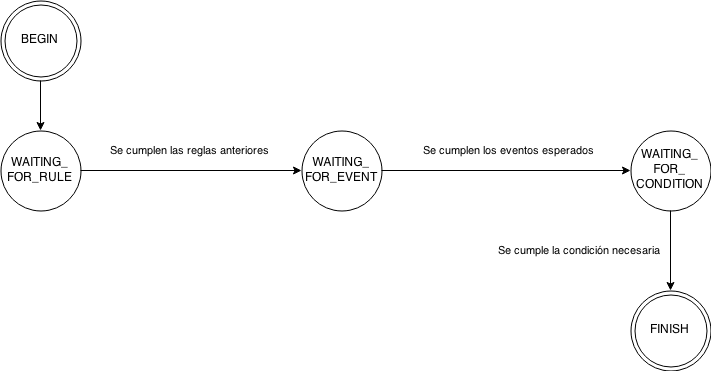
\includegraphics[width=12cm]{solucion/images/rules_flow.png}
\caption{Ciclo de vida de una regla}
\label{fig:rule_flow}
\end{figure}



Las reglas definidas dentro del procedimiento definen las acciones
que se deben llevar a cabo para completar el procedimiento, es necesario que
todas las reglas sean cumplidas para obtener un puntaje perfecto. Además definen el 
mecanismo que se utiliza para proveer una retroalimentación al usuario una vez finalizada 
la partida, pues cada regla almacena información acerca del progreso del usuario en cada paso.

%Cada regla contiene información acerca del estado del progreso del alumno en un
%paso en particular, estas reglas pueden tener como dependencias a otras reglas,
%es decir, una regla sólo se puede cumplir si una regla anterior se cumple, este
%es el caso de las reglas que definen la extracción de un torniquete, la cual
%depende de la regla que define la colocación del torniquete.  

En cuanto a la ejecución del motor de reglas, un motor de reglas \gls{eca} requiere de 
un proceso que evalúe constantemente
las reglas para verificar si las mismas deben ser lanzadas o
no\cite{bailey2004event,galton2002two}, un algoritmo comúnmente utilizado para
realizar la verificación es el algoritmo de \enquote{RETE}\cite{de2001eca}. La cantidad de
reglas definidas y la no dependencia circular entre ellas, hace innecesario la
implementación de tal algoritmo en este trabajo\cite{de2001eca}. 

De acuerdo a la descripción dada en~\ref{sec:eca}, la propuesta implementada
utiliza una ejecución inmediata, principalmente por la sencillez de las reglas,
es decir, las reglas no realizan un proceso complejo, solamente controlan el
estado del entorno y lo validan. Además, la ejecución inmediata es importante
por que el entorno no sufre modificaciones entre el evento lanzado y la
ejecución de la regla, según \cite{bailey2004event}, este es el factor más
importante para determinar el tipo de ejecución deseado.

El motor de reglas actúa sobre aquellas reglas en estado
\emph{WAITING\_FOR\_CONDITION} e invoca al procedimiento que se encarga de
validar si la regla puede ser activada (el procedimiento es único por cada
regla), si el mismo determina que la regla puede ser lanzada, el motor ejecuta
la acción de la regla y modifica el estado de la regla a \emph{FINISH}.


A continuación se muestran cada una de estas reglas definidas en la
tabla~\ref{tab:reglas_hemocultivo}, en donde se detallan cada uno de los estados
por los que pasa, a excepción de los estados BEGIN y FINISH que sólo indican el
inicio y fin de una regla. Una regla se cumple si se cumplen todas las reglas de
las cuales depende, si se lanzan los eventos esperados y si la condición del
entorno es la esperada.


\begin{table}[H]
\centering
\begin{tabulary}{\textwidth}{LLRRR}
\toprule
& Regla & Depende de las reglas & Espera a los eventos & Cuando se cumple que \\
\midrule
1  & Explicar procedimiento    &         & Explicar procedimiento    & Sea la primera regla lanzada\\
2  & Higienización de manos    & 1       & Higienización de manos    &\\
3  & Ponerse tababoca          & 2       & Ponerse tababoca          & Se realice antes de ponerse los guantes\\
4  & Ponerse gorro             & 2       & Ponerse gorro             & Se realice antes de ponerse los guantes\\
5  & Ponerse bata              & 2       & Ponerse bata              & Se realice antes de ponerse los guantes\\
6  & Calzar guantes            & 2,3,4,5 & Calzar guantes            &\\
7  & Colocar torniquete        & 10      & Colocar torniquete        & La zona correcta y mismo brazo de inserción\\
8  & Cerrar manos              & 7,10    & Cerrar puño               & Sea el mismo brazo que inserción\\
9  & Esterilizar zona          & 10      & Esterilizar zona          & Sea la misma zona que inserción\\
10 & Realizar punción          & 2       & Realizar punción          & Sea la zona correcta\\
11 & Retirar Torniquete        & 10,7    & Retirar Torniquete        & Sea el mismo torniquete que activo regla 7\\
12 & Abrir mano                & 10,8    & Abrir mano                & Sea la misma mano que activo regla 8\\
13 & Extraer Sangre            & 10,12   & Extraer Sangre            &\\
14 & Retirar Jeringa           & 10      & Retirar Jeringa           & Sea la misma jeringa que activo regla 10\\
15 & Presionar zona de punción & 10      & Presionar zona de punción & Sea la misma zona de punción\\
16 & Quitar tapaboca           & 10,3    & Quitar tapaboca           &\\
17 & Quitar gorro              & 10,4    & Quitar gorro              &\\
18 & Quitar bata               & 10,5    & Quitar bata               &\\
19 & Descalzar guantes         & 10,6    & Descalzar guantes         &\\
20 & Limpiar manos             & 19      & Limpiar manos             &\\
\bottomrule
\end{tabulary}
\caption{Reglas definidas para el procedimiento de extracción de sangre, se muestran los detalles de cada uno 
de los estados por los que pasan cada una de las reglas.}
\label{tab:reglas_hemocultivo}
\end{table}




\subsubsection{Retroalimentación y puntuación final}
\label{sec:puntuacion_hemocultivo}

Al final de una partida, la solución le brinda una retroalimentación al 
usuario como se muestra en la figura~\ref{fig:hemocultivo_retroalimentacion}.

\begin{figure}[H]
\centering 
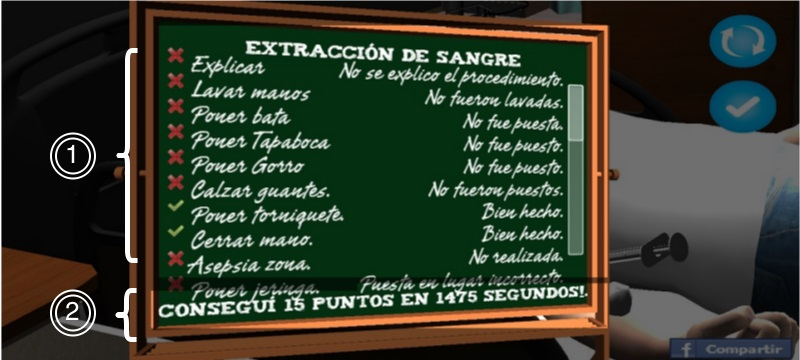
\includegraphics[width=10cm]{solucion/images/hemocultivo_retroalimentacion.jpg}
\caption{Retroalimentación y puntuación final del escenario \emph{Venopunción}.}
\label{fig:hemocultivo_retroalimentacion}
\end{figure}

En la parte $1$ de la figura~\ref{fig:hemocultivo_retroalimentacion}, se puede
ver como se brinda información al  usuario acerca de su rendimiento. Esta
información le indica los pasos que realizó de manera correcta o incorrecta y
las razones por las cuales tuvo ese desempeño.

Una regla puede quedar en uno de diferentes estados al final de la partida, cada
uno de esos estados posee un significado en el contexto del procedimiento y por
lo tanto tienen información asociada para brindar información al final de la
partida.

Cada paso en el procedimiento tiene asociado unos puntos, de acuerdo a la dificultad de realizar el
paso, estos puntos son utilizados al final de la partida para darle una puntuación al
usuario como se muestra en el punto $2$ de la
figura~\ref{fig:hemocultivo_retroalimentacion}. El puntaje final se obtiene sumando cada 
uno de los puntos logrados y calculando el porcentaje sobre el total que es de $27$. Junto al 
puntaje final se muestra el tiempo que le tomó al usuario completar el procedimiento.


\subsubsection{Registro de actividad}

Los eventos provocados por las acciones del usuario, la aplicación y el motor de 
reglas son registrados de manera transparente como se explica más adelante 
en~\ref{sec:backend_reg_eventos}. En la tabla~\ref{tab:hemocultivo_registro} se pueden observar los eventos relacionados al procedimiento.

%Existen otros tipos de eventos que no son generados por acciones, por ejemplo,
%cuando la simulación termina, el motor de reglas lanza un evento por regla,
%indicando su estado.
%
%El registro de actividades permite reproducir las \fixme{partidas}{Unificar
%    términos} y por lo tanto, es posible determinar que tareas \fixme{fueron con
%    las que los usuarios tuvieron}{pulir} un mayor número de inconvenientes.
%
%
%El registro de actividades se almacena en el dispositivo del usuario, y luego
%es enviado al \emph{backend}, esto se explica con más detalle
%en~\ref{sec:backend_reg_eventos}. 




\begin{table}[H]
\centering
\begin{tabulary}{\textwidth}{|L|L|L|}
\hline
Acción & Eventos & Motivos \\
\hline
Preparación del paciente & Explicación del procedimiento & Validación de interfaz intuitiva, 
de realización correcta de pasos y de la hipótesis \enquote{Interacción por la voz} \\
\hline
Bioseguridad inicial  & Lavado de manos, calzado de guantes, bata, tababoca y gorro & Validación 
de interfaz intuitiva, de realización correcta de los pasos y de la hipótesis 
\enquote{Bioseguridad} \\
\hline
Preparación para la extracción & Esterilización de zona, colocación de torniquete, petición de cierre de mano 
& Validación de interfaz intuitiva, de realización correcta de pasos y de validación de la hipótesis \enquote{Interacción por la voz} \\
\hline
Punción y extracción & Punzado, extracción de torniquete, petición de apertura de mano, extracción de sangre, 
extracción de jeringa & Validación de interfaz intuitiva, de realización correcta de pasos y de la 
hipótesis \enquote{Interacción por la voz} \\
\hline
Post - extracción & Presionar zona de punción & Interfaz intuitiva, realización correcta del paso \\
\hline
Bioseguridad final & Lavado de manos, descalzado de guantes, bata, tapaboca y gorro & Validación de interfaz intuitiva, de realización correcta de los pasos y de la hipótesis \enquote{Bioseguridad} \\
\hline
Utilización de redes sociales & Socialización del resultado de la partida & Medición del efecto motivador, validación de la hipótesis \enquote{Motivación}\\
\hline
\end{tabulary}
\caption{Acciones registradas durante una partida del procedimiento de venopunción, los eventos 
relacionados a ellas, y los motivos de sus registros.}
\label{tab:hemocultivo_registro}
\end{table}





\subsection{Valoración de la escala de Glasgow}

%\observacion{Más directo}
El escenario \emph{Valoración de la escala de Glasgow} se presenta en dos modos
distintos, en el primero, el usuario no conoce el estado del paciente, este modo
se conoce como \emph{Evaluar Glasgow}, y en su segundo, el usuario elige el
estado del paciente antes de iniciar la escena, este modo se conoce como
\emph{Exploración Glasgow}. 

%La reducida cantidad de diferencias entre ambos modos de la práctica permiten
%que ambas sean descritas en esta sección, las características explicadas son
%comunes para ambas, \fixme{salvo que se especifique lo contrario}{?}.

En el modo \emph{Exploración Glasgow}, antes de iniciar la escena, se le
permite al usuario seleccionar el estado del paciente mediante una interfaz 
como se puede observar en la figura~\ref{fig:glasgow_seleccion}, en
cambio, en el modo \emph{Evaluar Glasgow}, el estado del paciente no se conoce
de antemano y será responsabilidad del usuario determinarlo.

\begin{figure}[H]
\centering
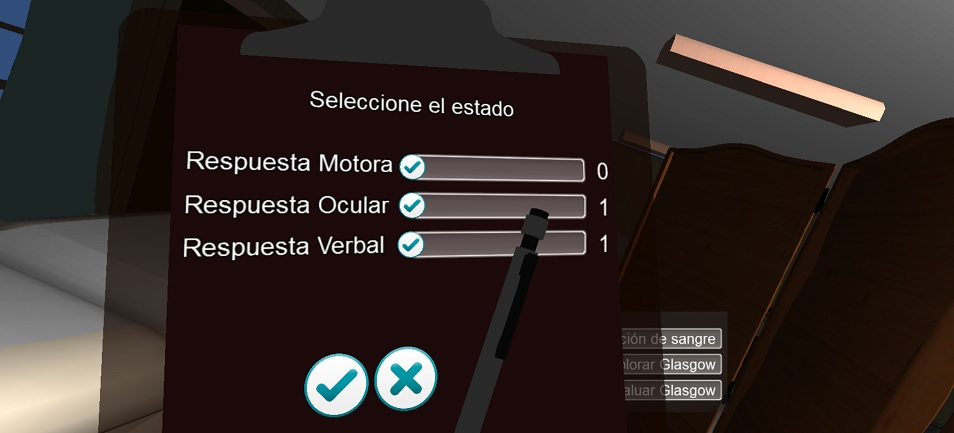
\includegraphics[width=10cm]{solucion/images/glasgow_seleccion.jpg}
\caption{Interfaz del modo \emph{Exploración Glasgow} para seleccionar el estado del 
paciente.}
\label{fig:glasgow_seleccion}
\end{figure}

%La pantalla principal de este procedimiento se muestra en la
%figura~\ref{fig:glasgow_principal}, en ella además de contar con el paciente sólo se ofrece
%una opción para finalizar la partida actual.

%\begin{figure}[H]
%\centering
%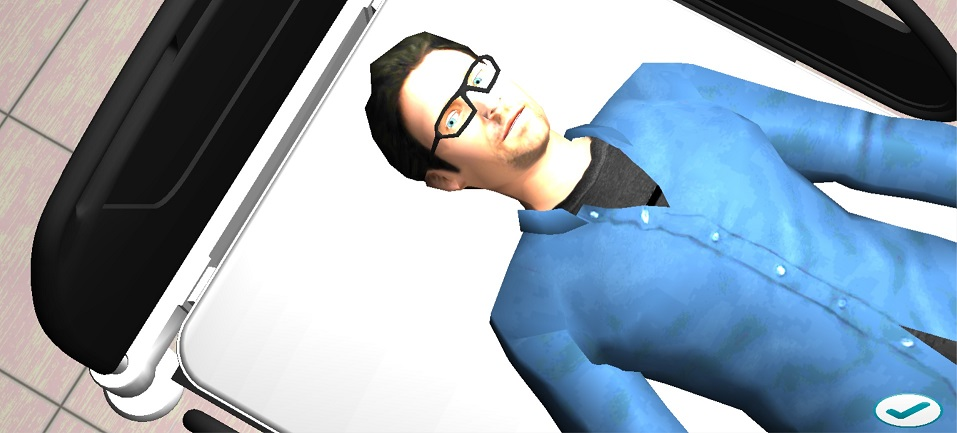
\includegraphics[width=10cm]{solucion/images/glasgow_principal.jpg}
%\caption{Pantalla principal de la escena de valoración de la escala de Glasgow.}
%\label{fig:glasgow_principal}
%\end{figure}



\subsubsection{Entidades}

%\observacion{Si la sección se llama entidades por que resalta otra cosa?}

Existen dos entidades principales, el usuario o \emph{Enfermero} y el \emph{Paciente}, 
el enfermero no almacena información, y el
paciente sólo almacena su estado, que se define al inicio. De esta forma, las
entidades no se modifican en ningún momento.

La información almacenada por la entidad paciente es su estado motor, verbal y
ocular, el cual es un conjunto de números, cuyos posibles valores se definen en
en~\ref{sec:glasgow_protocolo}, la definición de estos números varían de acuerdo
al modo de la escena como se describe a continuación:

\begin{itemize}
    \item Exploración: el usuario selecciona el estado que desea para el paciente, 
        este estado se mantendrá constante durante toda la partida.
    \item Evaluación: al inicio se crean tres números de manera
        aleatoria, el algoritmo que crea estos valores, lo hace de tal manera
        que el estado del paciente es consistente, por ejemplo, el paciente
        nunca tendrá un estado verbal \enquote{Orientado} (valor 5 en la escala)
        y un estado ocular \enquote{Ausente} (valor 1 en la escala), pues esto
        no tendría sentido, si no puede abrir los ojos (estado
        \enquote{ausente}), no puede saber donde esta (estado
        \enquote{orientado}). El estado se mantendrá constante durante toda partida.
\end{itemize}

Aunque el estado de las entidades no se modifique, esto no significa que no
puedan realizar acciones entre ellas, sino que estas acciones y los eventos
generados no alteran el estado de las entidades.


\subsubsection{Interacción con la interfaz de usuario} 

La interfaz de usuario, como se observa en la figura~\ref{fig:glasgow_principal}, es
muy sencilla, se compone de solo una opción permanente, la cual permite al
usuario finalizar la partida. Además se ve en la interfaz, al paciente, que es el 
foco principal de la cámara.
%Se observan además, las opciones que se despliegan cuando la solución detecta que
%el usuario emite palabras, conocidas como \emph{Comandos de Voz}, que permiten
%al usuario o enfermero interactuar con el paciente.

\begin{figure}[hbt]
\centering
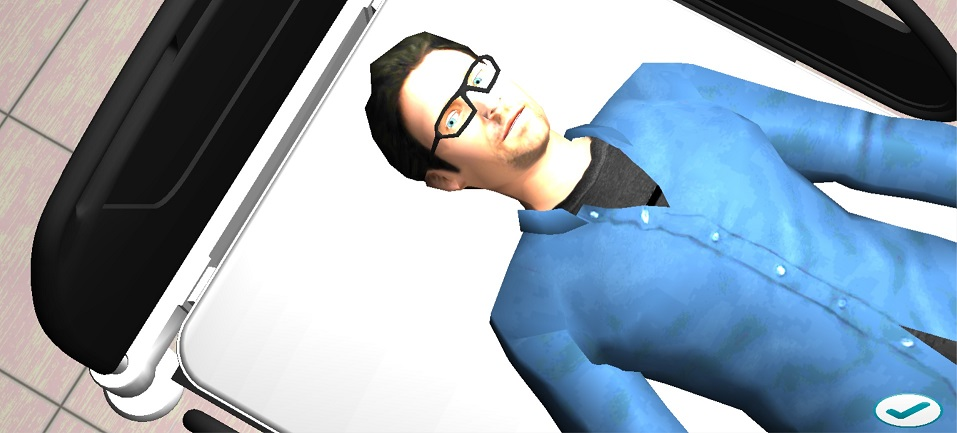
\includegraphics[width=10cm]{solucion/images/glasgow_principal.jpg}
\caption{Interfaz principal de la escena \emph{Evaluación de Glasgow}, se observa además
    la opción que permite finalizar la escena.}
\label{fig:glasgow_principal}
\end{figure}

El usuario puede interactuar con el paciente de dos modos, por un \enquote{menú
    de comandos de voz} y por opciones a través de \enquote{menú contextual}. 

\begin{itemize}

\item{\textbf{Menú Contextual}:} las opciones a través del menú contextual se
    relacionan a acciones que puede realizar el enfermero sobre una parte
    particular del cuerpo del paciente, en las extremidades, el menú despliega
    una sola opción, la cual es \emph{Pinchar} como se observa en la
    figura~\ref{fig:glasgow_menu_accion}, que provoca que el enfermero realice
    un estímulo doloroso al paciente. El paciente reacciona ante este estímulo
    dependiendo de su valoración motora y ocular. 

    \begin{itemize}
    \item Si el estado ocular del paciente es \enquote{Al dolor}, el paciente
        abrirá los ojos inmediatamente después de que se presione la opción. 
    \item  La respuesta motora varía de acuerdo a su estado, si el mismo es
        \enquote{Localiza}, el paciente mueve sus manos hasta el origen del
        dolor, si el estado es \enquote{Retira}, moverá la extremidad que
        sufrió el estímulo lejos de su posición inicial, si es
        \enquote{Flexión anormal}, el paciente reaccionará comprimiendo el
        cuerpo, indistintamente de la ubicación del estímulo doloroso, y si el
        estado es \enquote{Extiende}, el paciente extenderá el cuerpo también 
        indistintamente de la ubicación del estímulo doloroso.
    \end{itemize}

\begin{figure}[hbt]
\centering
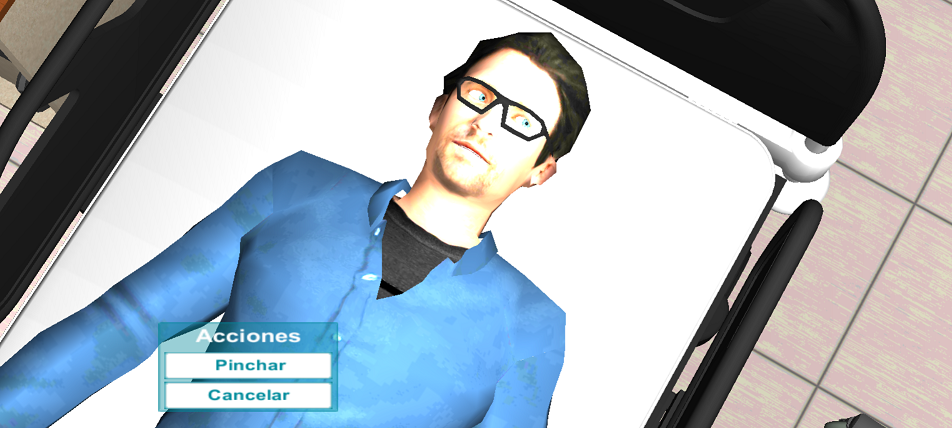
\includegraphics[scale=0.5]{solucion/images/glasgow_menu_accion.png}
\caption{Menú contextual para realizar un estímulo doloroso al paciente en el procedimiento de 
\emph{Valoración de la escala de Glasgow}.}
\label{fig:glasgow_menu_accion}
\end{figure}

\item{\textbf{Menú de comandos de voz}}

\begin{figure}[hbt]
\centering
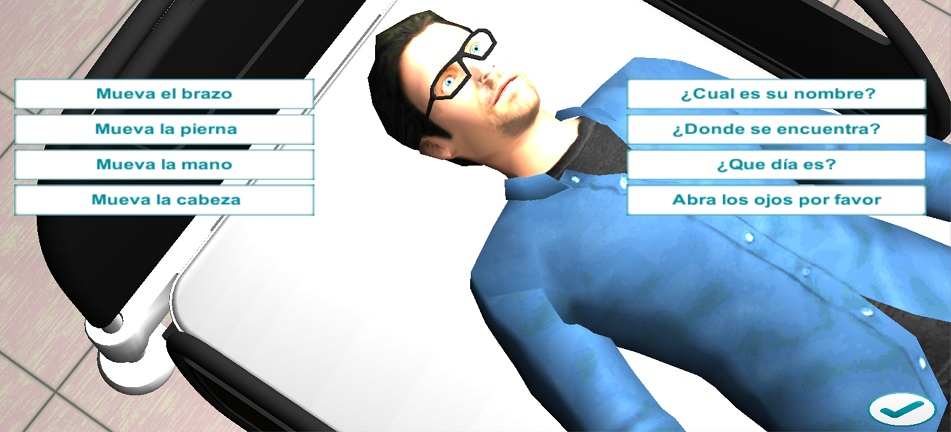
\includegraphics[scale=0.5]{solucion/images/glasgow_comandos_voz.jpg}
\caption{Interfaz de la escena \emph{Evaluación de Glasgow}, se observan los
    \emph{comandos de voz}, así como la opción que permite finalizar la escena
    (esquina inferior derecha).}
\label{fig:glasgow_gui}
\end{figure}

Las opciones del menú por comandos de voz del tipo \emph{motor}, son cuatro: 

\begin{itemize}
    \item Mueva el brazo
    \item Mueva la pierna
    \item Mueva la mano
    \item Mueva la cabeza
\end{itemize}

Estas opciones no tienen una respuesta sonora, en cambio, si el estado motor del paciente es
\enquote{Obedece}, este reacciona moviendo una extremidad, en caso
contrario, el paciente no realiza acción alguna.

Entre los comandos de voz existe una sola opción \emph{ocular}, la cual es 
\enquote{Abra sus ojos por
favor}, esta petición no tiene una respuesta sonora, y sólo si el paciente tiene un
estado ocular \enquote{Al hablar} abre los ojos, en caso contrario, no realiza
acción alguna.

Las preguntas y posibles respuestas de tipo \emph{verbal}, se pueden ver en la
tabla~\ref{tab:glasgow_opciones_respuesta}. 

\begin{table}[H]
\centering
\begin{tabulary}{\textwidth}{LCCCCC}
\toprule
\textbf{Pregunta} & \textbf{Orientado} & \textbf{Confusa} & \textbf{Palabras
    inapropiadas} & \textbf{Palabras incomprensibles} & \textbf{Ausente} \\
\midrule
¿Qué día es? & El día de la semana actual & Cualquier día de la semana menos el
correcto & La respuesta a otra pregunta en estado orientado & Gritos, gruñidos y
quejidos & No emite sonido \\
¿Cuál es su nombre? & \emph{Carlos Benitez} & Respuesta coherente sin mencionar
su nombre & Respuesta a otra pregunta en estado orientado & Gritos, gruñidos y
quejidos & No emite sonido \\
¿Donde se encuentra? & \emph{En una cama de hospital} & \emph{En mi dormitorio} &
Respuesta a otra pregunta en estado orientado & Gritos, gruñidos y quejidos & No
emite sonido \\
\bottomrule
\end{tabulary}
\caption{Posibles respuestas de acuerdo al estado verbal del paciente.}
\label{tab:glasgow_opciones_respuesta}
\end{table}

\end{itemize}

\subsubsection{Evaluación al usuario}
\label{sec:puntuacion_glasgow}

La evaluación del desempeño del usuario en la partida sólo se da en el modo \emph{Evaluación 
Glasgow}. %A continuación se describe el método de evaluación del procedimiento 
%de valoración de la escala  de Glasgow, se empieza describiendo como el 
%usuario registra su valoración en la solución.

Una vez que el usuario decida que está listo para dar un diagnóstico, procede a
finalizar la partida, en ese momento se presenta una pantalla donde el mismo
puede diagnosticar al paciente, como se observa en la
figura~\ref{fig:glasgow_gui_resultados}.

\begin{figure}[H]
\centering
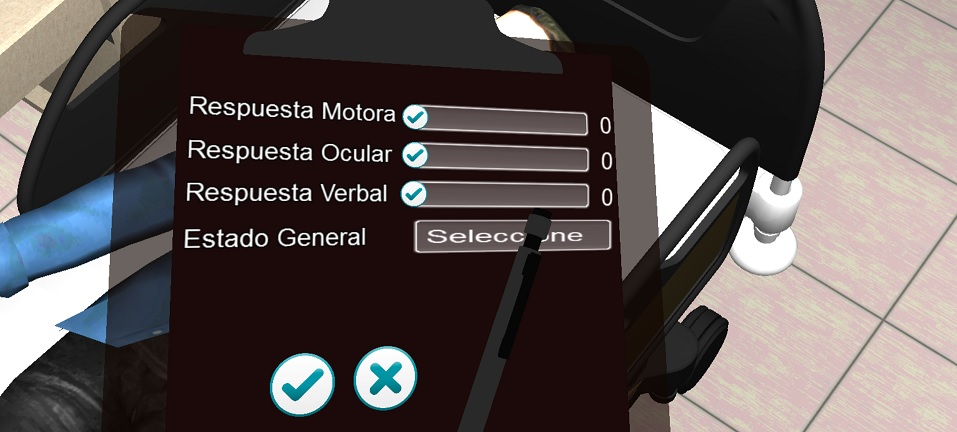
\includegraphics[width=10cm]{solucion/images/glasgow_diagnostico.jpg}
\caption{Vista de la \emph{Pantalla de diagnóstico}, donde el usuario puede
    asignar una puntuación a cada aspecto analizado del paciente.}
\label{fig:glasgow_gui_resultados}
\end{figure}

Las opciones presentadas al usuario son cuatro, puntuación verbal, ocular,
motora y un diagnóstico del estado general de conciencia del paciente. Los valores posibles 
se describen en~\ref{sec:glasgow_protocolo}.

El estado aleatorio del paciente que es generado al inicio de la partida es
guardado en una variable que no es modificada hasta que se reinicie la partida. 
Cuando el usuario confirma su diagnóstico la
aplicación lo compara con el estado guardado y de esta forma puede informar al
usuario acerca de su rendimiento en el diagnóstico. 

%\begin{itemize}
%\item{\textbf{Pantalla de diagnóstico}}
%
%Una vez que el usuario decida que está listo para dar un diagnóstico, procede a
%finalizar la partida, en ese momento se presenta una pantalla donde el mismo
%puede diagnosticar al paciente, como se observa en la
%figura~\ref{fig:glasgow_gui_resultados}.
%
%\begin{figure}[H]
%\centering
%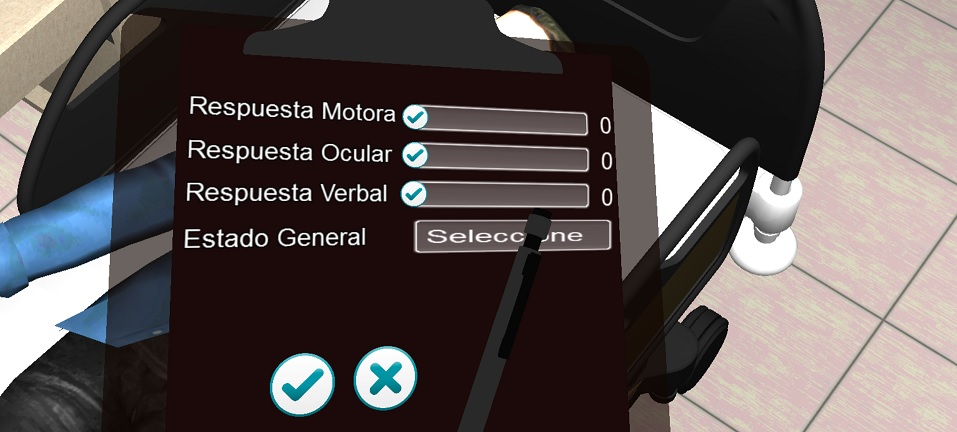
\includegraphics[width=10cm]{solucion/images/glasgow_diagnostico.jpg}
%\caption{Vista de la \emph{Pantalla de diagnóstico}, donde el usuario puede
%    asignar una puntuación a cada aspecto analizado del paciente.}
%\label{fig:glasgow_gui_resultados}
%\end{figure}
%
%Las opciones presentadas al usuario son cuatro, puntuación verbal, ocular,
%motora y un diagnóstico del estado general de conciencia del paciente. Los valores posibles 
%se describen en~\ref{sec:glasgow_protocolo}.
%
%\item{\textbf{Retroalimentación y puntuación final}}

\subsubsection{Retroalimentación y puntuación final}
%
%El estado aleatorio del paciente que es generado al inicio de la partida es
%guardado en una variable que no es modificada hasta que se reinicie la partida.
%Al final de la partida, la aplicación pide al usuario que valore el estado del
%paciente que le fue presentado, una vez que el usuario confirme su respuesta la
%aplicación la compara con el estado guardado y de esta forma puede informar al
%usuario acerca de su rendimiento en el diagnóstico. 

Cada posible respuesta dada por el usuario contiene información
relacionada al contexto del procedimiento y a la situación actual presentada, la
cual, es utilizada como retroalimentación al final de la partida como puede
verse en la figura~\ref{fig:glasgow_resultado} marcado por el número $1$. 

Para el cálculo del puntaje final que se le mostrará al usuario, por cada
respuesta dada en la pantalla de diagnóstico se asigna una puntuación de acuerdo
a que tan cerca estuvo el usuario de la respuesta correcta. Al final, se suman
estos valores y se calcula el porcentaje de acierto. El puntaje final junto a el
tiempo que tardó el usuario realizando el procedimiento se presenta como se
muestra en la figura~\ref{fig:glasgow_resultado} marcado por el número $2$.

\begin{figure}[H]
\centering
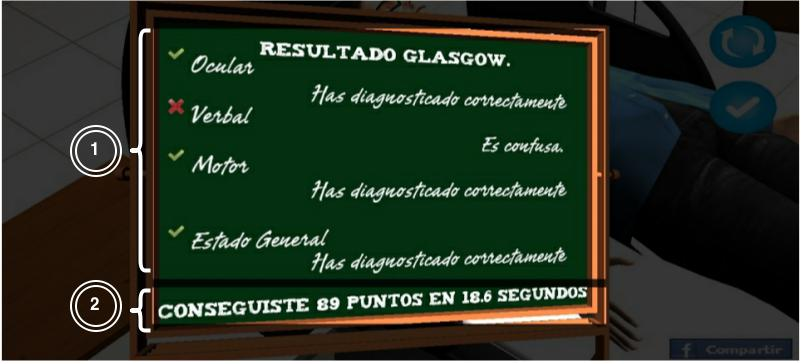
\includegraphics[width=10cm]{solucion/images/glasgow_resultado.jpg}
\caption{Retroalimentación y puntuación final del procedimiento de valoración de 
la escala de Glasgow.}
\label{fig:glasgow_resultado}
\end{figure}

%\end{itemize}

\subsubsection{Registro de actividad}
%\observacion{Todo esto es repetido}

Los eventos provocados por las acciones del usuario y por la aplicación son registrados de 
manera transparente como se explica más adelante en~\ref{sec:backend_reg_eventos}. En la 
tabla~\ref{tab:glasgow_registro} se pueden observan los eventos registrados.

%Cada acción que realiza el usuario dentro de la simulación provoca un evento, y
%estos eventos son registrados de manera transparente para el usuario. Como así
%también los eventos que genera la aplicación.
%
%El registro de actividades permite reproducir las partidas y por lo tanto, es
%posible determinar que tareas fueron con las que los usuarios tuvieron un mayor
%número de inconvenientes.



\begin{table}[H]
\centering
\begin{tabulary}{\textwidth}{|L|L|L|}
\hline
Acción & Eventos & Motivos \\
\hline
Estímulos dolorosos & Estimulación de extremidades del paciente & Validación de interfaz intuitiva \\
\hline
Acciones de voz  & Solicitudes y preguntas al paciente & Validación de la hipótesis \enquote{Interacción 
por la voz} \\
\hline
Diagnóstico del paciente & Valoración del usuario acerca de la respuesta motora, verbal y ocular 
del paciente así como su estado general & Validación de interfaz intuitiva, de realización correcta de 
la valoración \\
\hline
Utilización de redes sociales & Socialización del resultado de la partida & Medición del efecto motivador 
y validación de la hipótesis \enquote{Motivación}\\
\hline
\end{tabulary}
\caption{Acciones registradas durante una partida del procedimiento de valoración de la ecala 
de Glasgow, los eventos relacionados a ellas, y los motivos de sus registros.}
\label{tab:glasgow_registro}
\end{table}

%\observacion{Hay que depurar las cosas repetidas (esto esta abajo del primer
%párrafo de interfaz, pero me parece que incluye a las dos sub subsection)}

%\subsubsection{Interfaz de usuario}

%La interfaz de usuario, como se observa en la figura~\ref{fig:glasgow_gui}, es
%muy sencilla, se compone de solo una opción permanente, la cual permite al
%usuario finalizar la escena y mostrar la \emph{Pantalla de diagnóstico}. Se
%observan además, las opciones que se despliegan cuando la solución detecta que
%el usuario emite palabras, conocidas como \emph{Comandos de Voz}, que permiten
%al mismo interactuar con el paciente.
%
%\begin{figure}[H]
%\centering
%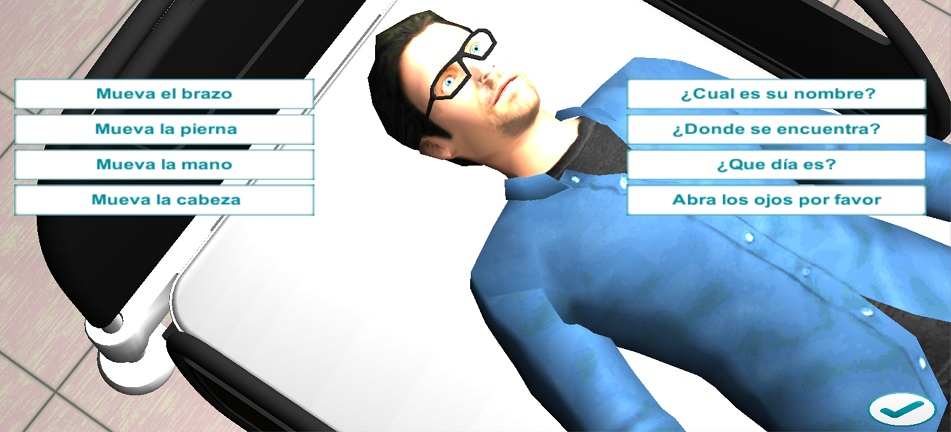
\includegraphics[scale=0.5]{solucion/images/glasgow_comandos_voz.jpg}
%\caption{Interfaz de la escena \emph{Evaluación de Glasgow}, se observan los
%    \emph{comandos de voz}, así como la opción que permite finalizar la escena
%    (esquina inferior derecha).}
%\label{fig:glasgow_gui}
%\end{figure}
%
%Además se ve en la interfaz, al paciente, que es el foco principal de la cámara.

\subsection{Pantalla de resultados}

Al finalizar tanto el escenario de \emph{Venopunción} como el escenario de \emph{Valoración de 
la escala de Glasgow}, se presenta una pantalla de resultados, la cual es
la encargada de mostrar toda la información que fue recabada durante la partida,
esta información incluye los pasos correctos e incorrectos que realizó el
usuario.

\begin{figure}[H]
\centering
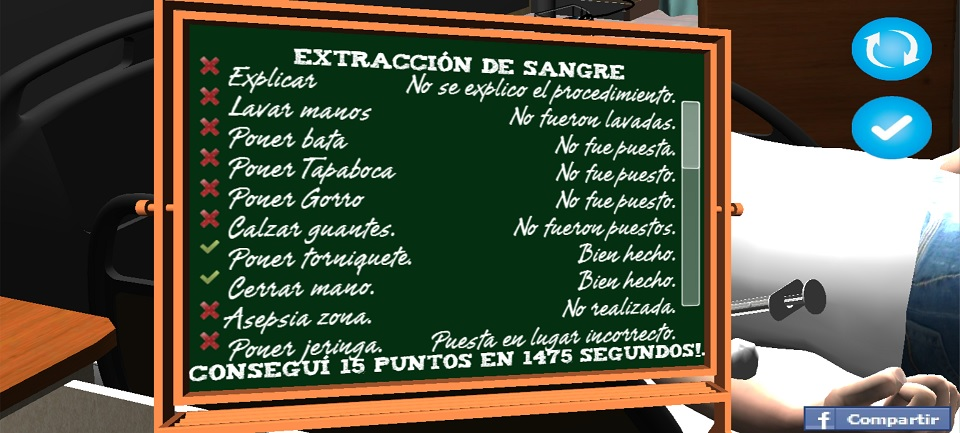
\includegraphics[scale=0.5]{solucion/images/resultado_hemocultivo.jpg}
\caption{Pantalla de resultados mostrando los pasos correctos e incorrectos, en
    la escena \emph{Glasgow}.}
\label{fig:resultados_glasgow}
\end{figure}

En la figura~\ref{fig:resultados_glasgow} se observa el diseño de la
pantalla, el título es la escena actual, un resumen de la
puntuación, y el tiempo que duró la partida.

Adicionalmente a la información de la sesión, se permite al usuario reiniciar la
partida, ir al menú de inicio, y compartir sus logros en las redes sociales.

Si el usuario presiona el botón \enquote{Facebook}, se despliega el menú de
dicha red social, permitiendo que el mismo pueda agregar un mensaje
personalizado y el resultado de la sesión se comparta con un texto similar a
\enquote{Conseguí 15 puntos en 1475 segundos, en el procedimiento de
    \emph{Venopunción} jugando con \textit{eTes\~{a}i}}.

